\documentclass[cjk]{beamer}
\usepackage{CJK}
\usepackage{latexsym, amsfonts, amssymb, amsmath,  amsthm}
\usepackage{amsopn, amstext, amscd,pifont}
\usepackage{amssymb,bm}
\usepackage{braket}
\usepackage{cases}
\usepackage{paralist}
\usepackage{eufrak}
\usepackage[all]{xy}
\usepackage[overload]{textcase}


%\useoutertheme[height=1.5em]{sidebar}

\logo{
\includegraphics[scale=0.09]{nuslogo.pdf}}

\usetheme{Berkeley}
\usecolortheme{seahorse}
%\usecolortheme{dove}

%\usefonttheme{professionalfonts}

\newtheorem{thm}[theorem]{Theorem}
\newtheorem{exa}[theorem]{Example}


\begin{document}

\title{On quantiles of Brownian motion and \\
quantile options}
\author{Zhu Yong Ting}
\date{} \frame{\titlepage}

\section{Agenda}
\begin{frame}
\frametitle{Organization of this Thesis}

\begin{itemize}
\item Introduction  $\color{red}\surd$
\item Principles of option pricing 
\item Numerical methods
\item Quantile and quantile options $\color{red}\surd$
\item Conclusion and future work $\color{red}\surd$
\end{itemize}
\end{frame}

\section{Introduction} 
\begin{frame}
\frametitle{Introduction}
Definition of quantiles:
for a stochastic process \{$X_t$\} on $(\Omega, \mathbb Q, \mathcal F)$, \\
\[
M(\alpha,t)(\omega) = \inf\Set{x:\int_0^t ds1_{(X_s (\omega)\leq x)} > \alpha t}.
\]
is the corresponding $\alpha$-quantile $(0 \leq \alpha \leq 1)$ process.
\vspace{1em}

Quantile options:
Just replace the spot price by the quantiles.

E.g. pay off function of 
\begin{itemize}
\item 
$\alpha$-quantile Eurpean call option: $(S(\alpha,T)-K)^+$;
\item 
$\alpha$-quantile Eurpean call option: $(S(\alpha,\tau)-K)^+$.
% when execrice the option at time \tau
\end{itemize}
\end{frame}

\section{Quantile}
\begin{frame}{Quantiles of Brownian motion}
Properties:
\begin{itemize}
\item $\displaystyle\inf_{0\leq s \leq t}  X_s = \lim_{\alpha\to 0}M(\alpha,t)$
\item $\displaystyle\sup_{0\leq s \leq t} X_s = \lim_{\alpha\to 1} M(\alpha, t)$.
\end{itemize}
\vspace{1em}

Now assume $X_t$ is a Brwonian motion.

Key property:
\[
(M(\alpha,T),X_T) 
{\stackrel{\text{(law)}}{=}}
 (\max_{t\leq \alpha T}X_t+\min_{t\leq (1-\alpha)T}X'_t, X_{\alpha T}+X'_{(1-\alpha)T}),
\]
where $X'_t$ is an independent copy of $X_t$. 
\end{frame}

\section{Discrete v.s. Continous}
\begin{frame}{Discretization}
Discretize the continous stochstics proscess(Brownian motion)
\[
X_{i,h} = X_{ih}
\]
is a discrete stochastic process(Gaussian randon walk),
 where $h$ is the step length.


$M_h(\alpha,T)$: the $k=\alpha T/h$-th order statistic of the set 
$\Set{X_{i,h}|n=0,1,\cdots, T/h}$.

Similar property ($h=T/N$,$k=\alpha N$)
\[
(M_h(1,T),X_{N,h}) 
{\stackrel{\text{(law)}}{=}}
 (\max_{i\leq k}X_{i,h}+\min_{i\leq N-k}X'_{i,h}, X_{k,h}+X'_{N-k,h}),
\]
\end{frame}

\begin{frame}{Discretization Error}
$Y$ is a random variable, $Y_h$ is a series of random variables prametrized by $h$. 

Different type of onvergence order: ($h\to 0$)
\begin{itemize}
\item {\em Strong order:} 
  \[
  \mathbb{E}\left|Y_h(t) - Y_h\right| \sim O(h^\gamma)
  \]
\item {\em Weak order:}
  \[
  \left|\mathbb{E} g(Y_h(t)) - g(Y_h)\right|  \sim O(h^\gamma), 
  \quad \forall g\in C^{2(\gamma+1)}(\mathbb{R})
  \]
\end{itemize}

\end{frame}

\begin{frame}{Results for maximal}
Running Maximal of Brownian motion: 
i.e. 
$\displaystyle Y = \max_{0\leq t\leq T} X_t, Y_h = \max_{0\leq i\leq T/h} X_{ih}$,\\
\em Strong and weak order of convergence is $1/2$ \cite{A-G-P-1995}. 

Moreover\cite{Janssen2008}, 
\[
\begin{split}
 & E[M(1,T)-M_{T/N}(1,T)]\\
=& -\frac{\zeta(1/2)}{\sqrt{2\pi}}\sigma\sqrt{T/N} 
 -\frac{2g(\mu\sqrt{T}/\sigma)-\mu\sqrt{T}/ \sigma}{4N}\sigma\sqrt{T} \\
 &+O(1/N^{3/2}),
\end{split}
\]
where
$g(x)=x \Phi(x) + \frac{1}{\sqrt{2\pi}} e^{-{x^2 /2 }}$,
and $\zeta$ is the Zeta-function, i.e. 
$
\zeta(1/2) \approx -3.92264613.
$

{\color{red} Question:} What about the quantiles.
\end{frame}

\begin{frame}{One result}
When $T/h \in \mathbb{N}$, we have 
\[
\mathbb{E}\left( M(\alpha, T) - M_h(\alpha,T)\right) 
= 
\begin{cases}
O(h^{1/2}) & \alpha=0,1\\
0 & \alpha=0.5\\
O(h) & \text{otherwize}
\end{cases} 
\]

Conclusion: The convergence patten of genuine $\alpha$-quantiles are different
with the extrema case. 
\end{frame}

\begin{frame}
\begin{figure}
   \centering
   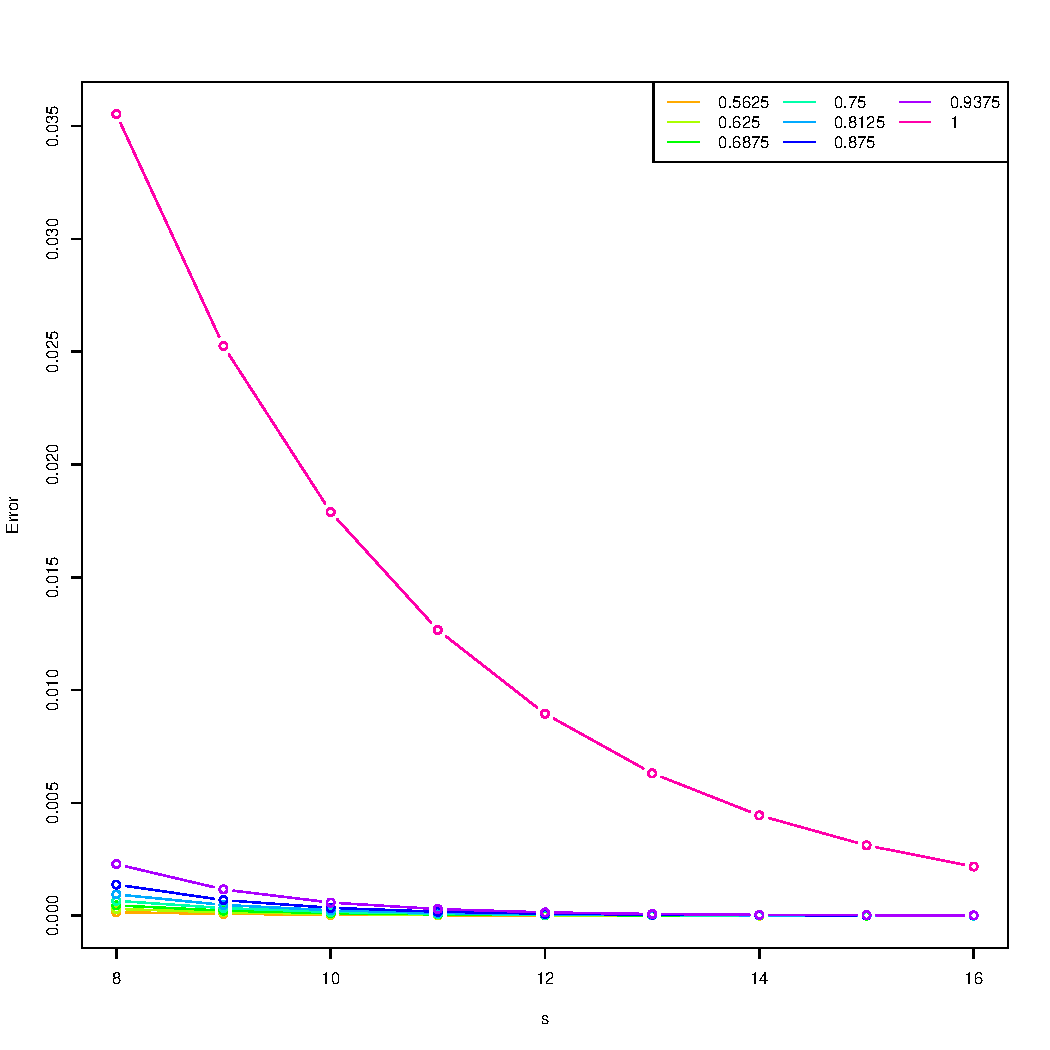
\includegraphics[scale=0.4]{nout_0.pdf} % requires the graphicx package
   \caption{Expectation of the discretization error for selected $\alpha$-quantile ($\alpha = 0.5625, 0.625, \cdots, 1$) using the Euler scheme with $N = 2^s$ ($4\le s \le 16$), $\mu=0$, $\sigma=1$, $T=1$, $X_0=0$, $L=500000$ }
   \label{f:err}
\end{figure}
\end{frame}

\begin{frame}
\begin{figure}
   \centering
   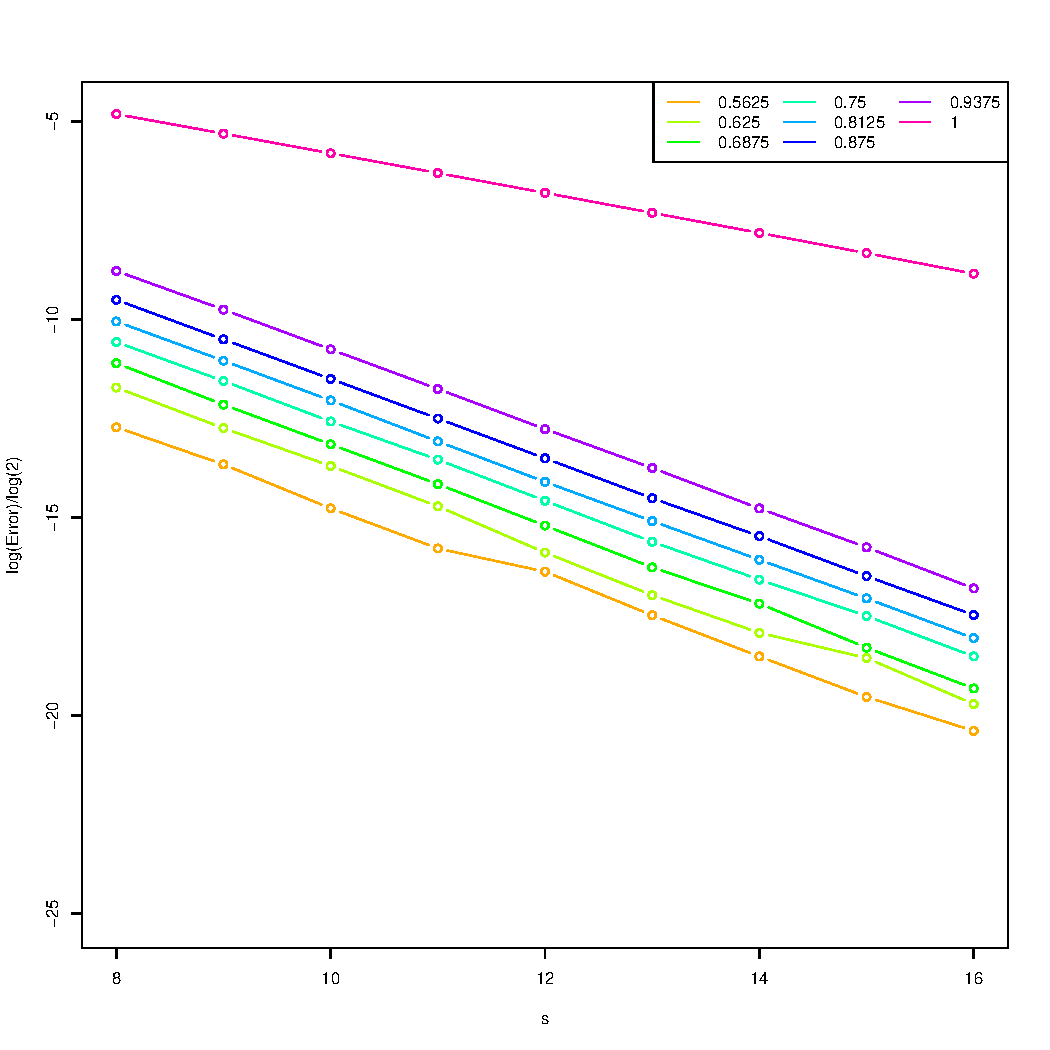
\includegraphics[scale=0.4]{nout_0log.pdf} % requires the graphicx package
   \caption{Logarithm of the discretization error for selected $\alpha$-quantile ($\alpha =$ $0.5625,$ $0.625,$ 
   $\cdots, 1$) using the Euler scheme with $N = 2^s$ ($4\le s \le 16$), $\mu=0$, $\sigma=1$, $T=1$, $X_0=0$, $L=500000$}
   \label{f:lerr}
\end{figure}
\end{frame}

\begin{frame}
\begin{figure}
   \centering
   \includegraphics[scale=0.4]{nout_0rato.pdf} % requires the graphicx package
   \caption{The order of convergence for selected $\alpha$-quantile ($\alpha = 0.5625, 0.625,  \cdots, 1$) using the Euler scheme with $N = 2^s$ ($4\le s \le 16$), $\mu=0$, $\sigma=1$, $T=1$, $X_0=0$, $L=500000$}
   \label{f:rate}
\end{figure}
\end{frame}


\begin{frame}{Numerical results for strong convergence order}
By numerical simulation, we also find a great differences of convergence pattens 
between genuine $\alpha$-quantiles are different
with the extrema case. 

\vspace{2em}
{\color{red}\em Conjecture:} For $\alpha\neq 0,1$, 
\[
\mathbb{E} |M(\alpha, T) - M_h(\alpha,T)|\sim O(h).
\]
\end{frame}

\begin{frame}
\begin{figure}
   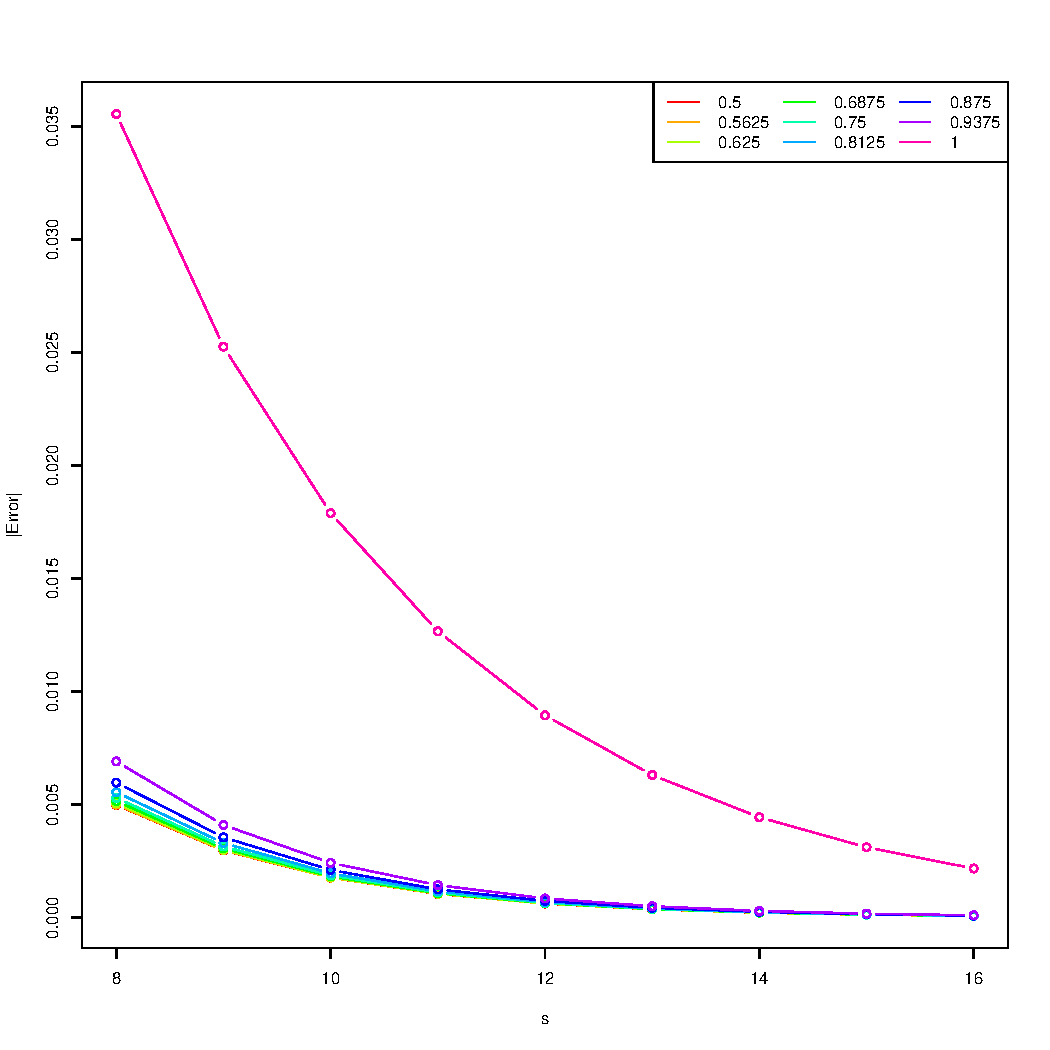
\includegraphics[scale=0.4]{nout_0a.pdf}
   \caption{Expectation of the absolute discretization error for selected $\alpha$-quantiles ($\alpha = 0.5, 0.5625, \cdots, 1$) using the Euler scheme with $N = 2^s$ ($4\le s \le 16$), $\mu=0$, $\sigma=1$, $T=1$, $X_0=0$ and $L=500000$. }
\label{f:ab}
\end{figure}
\end{frame}

\begin{frame}
 \begin{figure}
   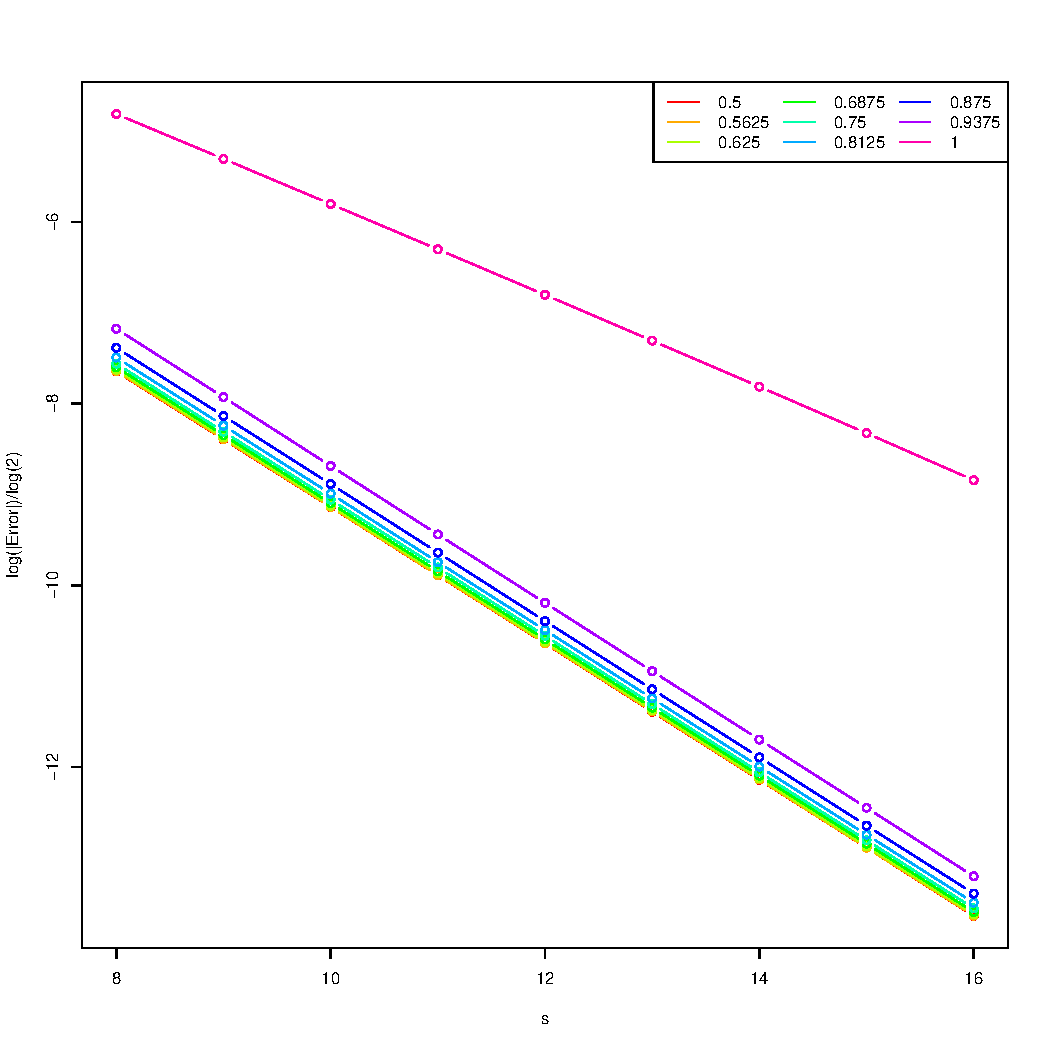
\includegraphics[scale=0.4]{nout_0alog.pdf}
   \caption{Logarithm of the absolute discretization error for selected $\alpha$-quantiles ($\alpha = 0.5, 0.5625, \cdots, 1$) using the Euler scheme with $N = 2^s$ ($4\le s \le 16$), $\mu=0$, $\sigma=1$, $T=1$, $X_0=0$, $L=500000$.} 
   \label{f:lab}
\end{figure}
\end{frame}

\begin{frame}
 \begin{figure}[p]
   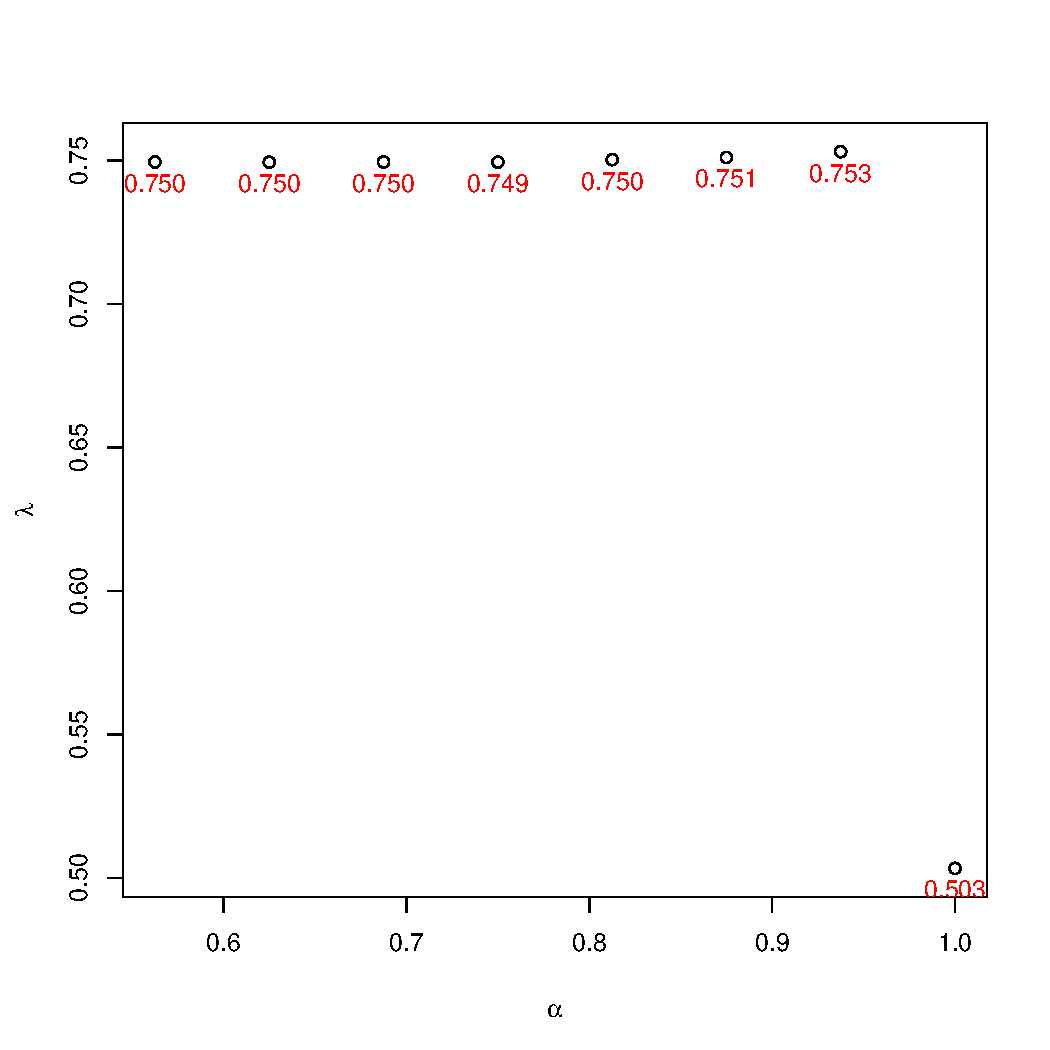
\includegraphics[scale=0.4]{nout_0arato.pdf} % requires the graphicx packagem 
   \caption{The strong order of convergence for selected $\alpha$-quantiles ($\alpha $ $=$ $ 0.5,$ $0.5625,$ $\cdots, 1$) using the Euler scheme with $N = 2^s$ ($4\le s \le 16$), $\mu=0$, $\sigma=1$, $T=1$, $X_0=0$, $L=500000$.}
   \label{f:ratio}
\end{figure}

\end{frame}

\section{Quantile Options}
\begin{frame}{Setting}
Under Black-Schorles's setting:\\
the price of undering assets 
satisfy a geometric Brownian motion. 
In fact, $S_t= S_0 e^{X_t}$, 
where $X_t$ is a Brownian motion with drift $r-\rho-\sigma^2/2$ 
and volatility $\sigma$,
let corresponding quantile process is 
$M(\alpha, t)$. 

We got the pricing formula, under Risk-Neutral framwork.
\end{frame}

\subsection{European}
\begin{frame}{Pricing formula}
Pay off at time $T$ of $\alpha$-quantile
\begin{itemize}
\item call option: $(S_0 e^{M(\alpha,T)} - K)^+$
\item put option: $(K - S_0 e^{M(\alpha,T)})^+$.
\end{itemize}

The price of European call option at any time $0\geq t\leq T$ is given by:
\[
V_t = \mathbb{E}\left(e^{-r(T-t)}(S_0 e^{M(\alpha,T)} - K)^+|\mathcal{F}_t\right)
\]

Discuss:\\
\begin{itemize}
\item For $t=0$, we can find $p_0$ by 
  \begin{itemize}
  \item closed formula with intergration \cite{Dassios1995},
  \item  efficient Monte Carlo simulation \cite{Laura2001}
  \item approximation by barriar option \cite{Kwok2001}.
  \end{itemize}
\item For $t> 0$, above methods do not work.  
\end{itemize}

We develop a tree method which can numerically price both European and American 
$\alpha$-quantile option at any time $t$.  
\end{frame}

%\subsection{Computational results for $\alpha$-quantile European option}
\begin{frame}{Numerical results for quantile European option}
\begin{table}
\caption{The price of European-style $\alpha$-quantile call options, with parameters
	$K=100, r=5\%, \sigma=0.2, \alpha=0.5, T=1$. }
\begin{center}
\begin{tabular}{l|lllllll}
 $S_0$ & $90$ & $95$ & $100$ & $105$ \\
\hline
28 steps & 1.60216 & 3.17876 & 5.61323 & 8.92661\\
30 steps & 1.60443 & 3.17806 & 5.61404 & 8.92702\\
32 steps & 1.60637 & 3.18346 & 5.61678 & 8.92718\\ 
34 steps & 1.60435 & 3.18426 & 5.61758 & 8.92875\\
36 steps & 1.60411 & 3.18846 & 5.61940 & 8.92925\\
\hline
Monte Carlo & 1.62450 & 3.21390 &  5.65385 & 8.96801 \\
Standard error & 0.00141 & 0.00200 & 0.00262 & 0.00317 \\
\hline
lookback & 9.45696 & 13.86499 & 19.16763 & 24.88215
\end{tabular}
\end{center}
\label{fig:euro5}
\end{table}%
\end{frame}

\begin{frame}{Numerical results for quantile European option}
\begin{table}
\caption{The price of European-style $\alpha$-quantile call option,
	with parameters
	$K=95, r=5\%, \sigma=0.2, \alpha=0.8, T=0.25$. }
\begin{center}
\begin{tabular}{l|lllllll}
$S_0$ & $95$ & $100$ & $105$        \\
\hline
26 steps & 4.59876 & 9.10824 & 14.1838 \\
28 steps & 4.60931 & 9.11777 & 14.1954 \\
30 steps & 4.61547 & 9.12485 & 14.2030 \\
32 steps & 4.61816 & 9.12648 & 14.2054 \\
34 steps & 4.61785 & 9.12676 & 14.2051 \\
36 steps & 4.62050 & 9.12908 & 14.2079 \\
\hline
Monte Carlo & 4.66740 & 9.18266 & 14.26175\\
Standard error & 0.00168 & 0.00200 &  0.00214\\
\hline
lookback & 8.381566 &  13.76059 & 19.13961
\end{tabular}
\end{center}
\label{fig:euro8}
\end{table}%
\end{frame}


\subsection{American}
\begin{frame}
Under the Risk-Neutral framwork, the price of $\alpha$-quantile American call option
is given by:
\[
V_t = \sup_{t \leq\tau\leq T}
\mathbb{E}\left(e^{-r(T-\tau)}(S_0 e^{M(\alpha,T)} - K)^+|\mathcal{F}_t\right)
\] 

{\em Discuss:}
\begin{itemize}
\item Typical optimal stopping problem
\item Discretized problem will give a an approximation solution of the original. 
\item The binomail tree method is doable, but no efficient.
\end{itemize}
\end{frame}

\begin{frame}{Computational results for $\alpha$-quantile American option}
\begin{table}[p]
\caption{The price of American-style $\alpha$-quantile call options, with parameter
	$K=100, r=0.05, \sigma=0.2, \alpha=0.5, T=1$. 
	%The extrapolation is based on results got at 28 steps and 36 steps.
	}
\begin{center}
\begin{tabular}{l|lllllll}
$S_0$ & $90$ & $95$ & $100$ & $105$ \\
\hline
26steps & 1.69411 & 3.43582 & 6.19546 & 10.2276 \\
28steps & 1.70066 & 3.44695 & 6.21365 & 10.2465 \\
30steps & 1.70434 & 3.45157 & 6.22887 & 10.2624 \\
32steps & 1.70651 & 3.45927 & 6.24320 & 10.2738 \\
34steps & 1.70590 & 3.46373 & 6.25529 & 10.2831 \\
36steps & 1.70711 & 3.47019 & 6.26644 & 10.2891 \\
%Extrapolation & 1.729685 & 3.551530 & 6.451205 & 10.43820 \\
\end{tabular}
\end{center}
\label{fig:amer5}
\end{table}
\end{frame}

\begin{frame}{Computational results for $\alpha$-quantile American option}
\begin{table}
\caption{The price of American-style $\alpha$-quantile call options, with parameters
	$K=95, r=5\%, \sigma=0.2, \alpha=0.8, T=0.25$. 
	%The extrapolation is based on results got at 28 steps and 36 steps.
	}
\begin{center}
\begin{tabular}{l|lllllll}
$S_0$ & $95$ & $100$ & $105$        \\
\hline
26 & 4.84702 &  9.68628 & 14.8771\\
28 & 4.85892 &  9.70169 & 14.8932\\
30 & 4.86696 &  9.71225 & 14.9049\\
32 & 4.87621 &  9.72318 & 14.9164\\
34 & 4.88228 &  9.73134 & 14.9251\\
36 & 4.88821 &  9.73857 & 14.9329\\
%extrapolation & 4.990725 & 9.867650&  15.07185
\end{tabular}
\end{center}
\label{fig:amer8}
\end{table}
\end{frame}

\subsection{The tree method}

\begin{frame}{Brief introduce of the tree method}
Similar to the usual binormial tree, but not connect the neighbor nodes.

\includegraphics[width=0.29\textwidth]{bitree.pdf}
\parbox[b]{0.7\textwidth}{
\begin{itemize}
\item depth $\leftrightarrow$ time; position $\leftrightarrow$ spot price 
\item Node $\leftrightarrow$ path 
\item Visit nodes by Depth-first search alg.
\item $Pay_{\text{Node}} = (S_{\text{Node}}-K)^+$
\item $V_{\text{Node}} = Pay_{\text{Node}}$ for all leaves.
\item $E_{\text{Node}} =$ discounted value of weighted avg. of 
  the $Pay$ of childerns.
\item $V_{\text{Node}} = \max\Set{Pay_{\text{Nod}}, E_{\text{Node}}} $
\item The price at time $t=0$ is $V_{\text{root}}$
\end{itemize}
}
\end{frame}

\section{Further directions}
\begin{frame}{Further directions}
\begin{itemize}
\item Proof the conjecture about the convergence patten of discretization error. 
\item Find efficient algorithm to price 
  the $\alpha$-quantile European and American option at any time $t$. 
\item Find certain connection of discrete and continous quantile options, 
  probably by using the conjecture. 
\end{itemize}
\end{frame}

\section{Reference}
\begin{frame}[allowframebreaks]{Reference}
\bibliographystyle{alpha}
\bibliography{prob}
\end{frame}

\end{document} 